\chapter{微分几何与对称性}
\label{chap:differential-geometry-and-symmetry}

前两章都在一个固定向量空间中讨论坐标。换基会改变数字表示，却不会改变向量、线性关系
和内积；谱与奇异值又说明，线性映射沿不同方向保留了多少信息。但许多数据并不接近一个
贯穿全局的低维线性子空间。一条一维曲线可以在环境空间中弯曲，观测点也可能在曲线周围
散开成有厚度的带。前者只有一个内在自由度，后者若被当作连续几何对象则有两个内在
自由度；测量噪声又是对潜在点的扰动，不会自动成为新的流形坐标。若不先分清这些对象，
“沿带移动”究竟允许哪些路径便没有确定含义。

本章以一条\term{弯曲点带}贯穿讨论。先考虑平面中的连续带
\begin{equation}
  \Phi(s,u)
  =
  \begin{bmatrix}
    (R+u)\cos(s/R)\\
    (R+u)\sin(s/R)
  \end{bmatrix},
  \qquad
  s\in I,\quad |u|<w<R,
  \label{eq:geometry-curved-strip-parameterization}
\end{equation}
其中$I=(s_-,s_+)\subset\mathbb{R}$是长度小于$2\pi R$的开区间，$s$表示沿中心线的位置，
$u$表示横向偏移。这个长度限制使参数化不会绕圆一周后重复。二维带和它的一维中心线
分别记为
\[
  \mathcal{M}_{\mathrm{strip}}
  =
  \{\Phi(s,u):s\in I,\ |u|<w\},
  \qquad
  \mathcal{C}
  =
  \{\Phi(s,0):s\in I\}.
\]
采样时，$\bm{p}_i=\Phi(s_i,u_i)\in\mathcal{M}_{\mathrm{strip}}$表示无噪声的
\term{潜在点}（latent point），
$\bm{x}_i=\bm{p}_i+\bm{\epsilon}_i\in\mathbb{R}^2$才是带测量误差的观测；
由于二维开带是$\mathbb{R}^2$的开子集，任一内部潜在点周围都有完全落在带内的小球，
足够小的扰动仍会使$\bm{x}_i\in\mathcal{M}_{\mathrm{strip}}$。没有噪声界时则不能
保证这一点，而且即使观测仍在带内，$\bm{x}_i$也不等于生成它的潜在点。若建模对象是
一维中心线，则还须令潜在点满足$u_i=0$，并把横向偏离归入观测误差；一般环境扰动会使
$\bm{x}_i\notin\mathcal{C}$，不能同时把$u$当作第二个内在坐标。后文将始终区分二维带
$\mathcal{M}_{\mathrm{strip}}$、一维中心线$\mathcal{C}$、潜在点$\bm{p}_i$和带噪
观测$\bm{x}_i$。

点间距离的嵌入与流形局部坐标解决两种表示问题：前者重构有限点集的欧氏坐标，后者描述
连续对象附近的自由度。切空间与局部内积随后共同定义路径长度、函数梯度和几何能量。
在这些局部工具之外，群作用研究指定变换下对象怎样对应，拓扑则研究整体连接与环。
对称性并非坐标不唯一就自动具备的任务性质，拓扑也不能由一个点的切空间判断；
这两条分支分别补充局部度量看不到的结构。所有结论都附带尺度、光滑性或采样条件；低维几何本身不保证它与某个预测任务
的语义一致。

\section{距离与坐标嵌入}
\label{sec:geometry-distance-coordinate-embedding}

\subsection{距离与坐标自由度}

先考虑$n$个无噪声点$\bm{y}_1,\ldots,\bm{y}_n\in\mathbb{R}^d$，将它们按行组成矩阵
$\bm{Y}\in\mathbb{R}^{n\times d}$。这些点可以取为前述潜在点；若把带噪观测直接
代入，以下结论只会重构观测距离，而不会自动恢复潜在距离。沿用定义~\ref{def:linear-algebra-gram-matrix}，点的\term{Gram矩阵}记录
两两内积：
\[
  \bm{B}=\bm{Y}\bm{Y}^{\top},
  \qquad
  b_{i,j}=\bm{y}_i^{\top}\bm{y}_j.
\]
若已知$\bm{B}$，平方距离可以由
\begin{equation}
  \delta_{i,j}
  =
  \lVert\bm{y}_i-\bm{y}_j\rVert_2^2
  =
  b_{i,i}+b_{j,j}-2b_{i,j}
  \label{eq:geometry-distance-from-gram}
\end{equation}
得到。反向恢复却多一个困难：距离不记录原点。把每个点同时平移
$\bm{a}\in\mathbb{R}^d$，全部差向量和距离都不变，内积却通常改变。

可以先选择一个规范来消除平移自由度。本节把点云中心放在原点，即要求
$\sum_i\bm{y}_i=\bm{0}$。令$\bm{1}\in\mathbb{R}^n$为全一向量，并定义中心化矩阵
\begin{equation}
  \bm{J}
  =
  \bm{I}_n-\frac{1}{n}\bm{1}\bm{1}^{\top}.
  \label{eq:geometry-centering-matrix}
\end{equation}
它满足$\bm{J}^{\top}=\bm{J}$、$\bm{J}^2=\bm{J}$和$\bm{J}\bm{1}=\bm{0}$，
所以是到与$\bm{1}$正交的子空间上的投影。对任意点矩阵，$\bm{J}\bm{Y}$恰好从每一行
减去样本均值。

把平方距离组成矩阵
$\bm{\Delta}\in\mathbb{R}^{n\times n}$，其中
$\Delta_{i,j}=\delta_{i,j}$。式~\eqref{eq:geometry-distance-from-gram}可写成
\[
  \bm{\Delta}
  =
  \operatorname{diag}(\bm{B})\bm{1}^{\top}
  +
  \bm{1}\operatorname{diag}(\bm{B})^{\top}
  -
  2\bm{B}.
\]
在左右两侧同时乘$\bm{J}$时，前两项因
$\bm{J}\bm{1}=\bm{0}$而消失。若点云已经中心化，则
$\bm{J}\bm{Y}=\bm{Y}$，从而$\bm{J}\bm{B}\bm{J}=\bm{B}$。于是得到
\begin{equation}
  \bm{B}
  =
  -\frac{1}{2}\bm{J}\bm{\Delta}\bm{J}.
  \label{eq:geometry-double-centering}
\end{equation}
这一步称为距离矩阵的\term{双重中心化}（double centering）。它不是把已有坐标投影
到某个子空间，而是从点间关系重新构造一组以均值为原点的内积。

\subsection{欧氏距离矩阵与半正定性}

任意实矩阵$\bm{Y}$产生的
$\bm{B}=\bm{Y}\bm{Y}^{\top}$都半正定，因为
\[
  \bm{c}^{\top}\bm{B}\bm{c}
  =
  \lVert\bm{Y}^{\top}\bm{c}\rVert_2^2
  \geq0.
\]
这个必要条件也是有限点欧氏嵌入的核心判据。

\begin{lemma}[双重中心化核的形式]
\label{lem:geometry-double-centering-kernel}
设$\bm{H}\in\mathbb{R}^{n\times n}$对称。若
$\bm{J}\bm{H}\bm{J}=\bm{0}$，则存在$\bm{a}\in\mathbb{R}^n$使
\[
  \bm{H}
  =
  \bm{1}\bm{a}^{\top}
  +
  \bm{a}\bm{1}^{\top}.
\]
若进一步有$h_{i,i}=0$对所有$i$成立，则$\bm{H}=\bm{0}$。
\end{lemma}

\begin{proof}
令$\bm{m}=\bm{H}\bm{1}/n$且
$\mu=\bm{1}^{\top}\bm{H}\bm{1}/n^2$。展开
$\bm{J}\bm{H}\bm{J}=\bm{0}$得到
\[
  \bm{H}
  =
  \bm{1}\bm{m}^{\top}
  +
  \bm{m}\bm{1}^{\top}
  -
  \mu\bm{1}\bm{1}^{\top}.
\]
取$\bm{a}=\bm{m}-(\mu/2)\bm{1}$便得到所需形式。此时
$h_{i,i}=2a_i$；若对角元全为零，则$\bm{a}=\bm{0}$，从而$\bm{H}=\bm{0}$。
\end{proof}

\begin{theorem}[有限距离的欧氏坐标重构]
\label{thm:geometry-euclidean-distance-embedding}
设$\bm{\Delta}\in\mathbb{R}^{n\times n}$对称、对角元为零，并令
\[
  \bm{B}
  =
  -\frac{1}{2}\bm{J}\bm{\Delta}\bm{J}.
\]
矩阵$\bm{\Delta}$是某组欧氏点的平方距离矩阵，当且仅当$\bm{B}$半正定。若
$r=\operatorname{rank}(\bm{B})$，则这些点可以嵌入$\mathbb{R}^r$，但不能嵌入
更低维的欧氏空间而精确保留全部距离。
\end{theorem}

\begin{proof}
若$\bm{\Delta}$来自欧氏点，先把点中心化。前面的双重中心化推导给出
$\bm{B}=\bm{Y}\bm{Y}^{\top}$，所以$\bm{B}$半正定。

反过来，若$\bm{B}$半正定，由谱定理可写
\[
  \bm{B}
  =
  \bm{Q}_r\bm{\Lambda}_r\bm{Q}_r^{\top},
\]
其中$\bm{\Lambda}_r$只保留$r$个正特征值。取
\begin{equation}
  \bm{Y}
  =
  \bm{Q}_r\bm{\Lambda}_r^{1/2},
  \label{eq:geometry-classical-scaling-coordinates}
\end{equation}
便有$\bm{Y}\bm{Y}^{\top}=\bm{B}$。由
$\bm{B}\bm{1}=\bm{0}$可知$\bm{Y}^{\top}\bm{1}=\bm{0}$，故坐标已经中心化。
用式~\eqref{eq:geometry-distance-from-gram}从$\bm{B}$构造平方距离，所得矩阵与
$\bm{\Delta}$有相同的双重中心化结果。两者之差是对称矩阵、对角元为零，且双重
中心化为零；引理~\ref{lem:geometry-double-centering-kernel}说明两者之差只能为零，
所以距离完全相同。

最后，任何坐标矩阵$\widetilde{\bm{Y}}\in\mathbb{R}^{n\times k}$产生的Gram矩阵
秩至多为$k$。要得到秩为$r$的$\bm{B}$，必有$k\geq r$；式
~\eqref{eq:geometry-classical-scaling-coordinates}又表明$k=r$可以达到。
\end{proof}

这个重构过程是经典尺度分析的代数核心。若$\bm{B}$有负特征值，给定关系便不能作为
欧氏平方距离被精确保留。实际计算有时只保留正特征值，得到近似坐标；此时舍弃负谱是一项
近似选择，不能把输出再称为原距离的精确实现。若各对距离分别带有测量误差，彼此可能不再
满足欧氏距离关系，双重中心化后便可能出现很小的负特征值；此时应结合误差尺度判断，而
不是见到负值就自动删除。若先获得一组带噪坐标再由它们精确计算成对距离，所得双重中心化
矩阵仍是这组观测坐标的Gram矩阵，因而不会仅因坐标噪声而失去半正定性。

\subsection{刚体变换与嵌入非唯一性}

即使$\bm{B}$半正定，重构坐标也不唯一。给定正交矩阵
$\bm{Q}\in\mathbb{R}^{r\times r}$与平移$\bm{a}\in\mathbb{R}^r$，令
\[
  \widetilde{\bm{y}}_i
  =
  \bm{Q}\bm{y}_i+\bm{a}.
\]
由于$\bm{Q}^{\top}\bm{Q}=\bm{I}$，
\[
  \lVert\widetilde{\bm{y}}_i-\widetilde{\bm{y}}_j\rVert_2
  =
  \lVert\bm{Q}(\bm{y}_i-\bm{y}_j)\rVert_2
  =
  \lVert\bm{y}_i-\bm{y}_j\rVert_2.
\]
正交矩阵既包括行列式为$1$的旋转，也包括行列式为$-1$的反射。距离因此不能确定绝对
位置、朝向或手性。中心化只固定平移，仍保留正交自由度；若特征值重复，谱分解中的单个
坐标轴还可以在相应子空间内任意旋转。

这也是中心化最小维坐标的全部不确定性。设
$\bm{Y},\widetilde{\bm{Y}}\in\mathbb{R}^{n\times r}$都列满秩、行均值为零，并产生
同一组距离。双重中心化给出
$\bm{Y}\bm{Y}^{\top}=\widetilde{\bm{Y}}\widetilde{\bm{Y}}^{\top}=\bm{B}$。
取$\bm{B}$的紧谱分解
$\bm{B}=\bm{Q}_r\bm{\Lambda}_r\bm{Q}_r^{\top}$。由于两组坐标的列空间都等于
$\bm{B}$的值域，定义
\[
  \bm{M}
  =
  \bm{\Lambda}_r^{-1/2}\bm{Q}_r^{\top}\bm{Y}.
\]
于是
\[
  \bm{Y}
  =
  \bm{Q}_r\bm{\Lambda}_r^{1/2}\bm{M},
  \qquad
  \bm{M}\bm{M}^{\top}
  =
  \bm{\Lambda}_r^{-1/2}
  \bm{Q}_r^{\top}\bm{Y}\bm{Y}^{\top}\bm{Q}_r
  \bm{\Lambda}_r^{-1/2}
  =
  \bm{I}_r.
\]
矩阵$\bm{M}$为方阵，所以它是正交矩阵。令$\bm{M}=\bm{U}^{\top}$，并对
$\widetilde{\bm{Y}}$作同样推导，可写成
\[
  \bm{Y}=\bm{Q}_r\bm{\Lambda}_r^{1/2}\bm{U}^{\top},
  \qquad
  \widetilde{\bm{Y}}
  =\bm{Q}_r\bm{\Lambda}_r^{1/2}\widetilde{\bm{U}}^{\top},
\]
其中$\bm{U}$和$\widetilde{\bm{U}}$均为$r$阶正交矩阵。因此
$\widetilde{\bm{Y}}=\bm{Y}\bm{U}\widetilde{\bm{U}}^{\top}$，两者只差一个作用在坐标
列上的正交变换。若允许更高维坐标，同一结论应理解为两组点在各自张成空间之间存在保距
正交对应，而多出的环境方向不含点云信息。

一个三点算例可以同时核对距离、Gram矩阵和非唯一性。取
\[
  \bm{y}_1=(-1,0)^{\top},\qquad
  \bm{y}_2=(0,1)^{\top},\qquad
  \bm{y}_3=(1,0)^{\top}.
\]
其平方距离矩阵为
\[
  \bm{\Delta}
  =
  \begin{bmatrix}
    0&2&4\\
    2&0&2\\
    4&2&0
  \end{bmatrix}.
\]
原坐标均值为$(0,1/3)^{\top}$。双重中心化恢复的是减去该均值后的Gram矩阵
\begin{equation}
  -\frac12\bm{J}\bm{\Delta}\bm{J}
  =
  \begin{bmatrix}
    10/9&-2/9&-8/9\\
    -2/9&4/9&-2/9\\
    -8/9&-2/9&10/9
  \end{bmatrix},
  \label{eq:geometry-three-point-centered-gram}
\end{equation}
其两个正特征值为$2$和$2/3$，所以精确欧氏嵌入至少需要二维。对重构坐标整体旋转或
反射仍得到同一$\bm{\Delta}$；把原坐标直接拿来比较时，还要补回任意平移。

弯曲点带展示了“重构”和“投影”的区别。若已经给出无噪声潜在坐标
$\bm{p}_i=\Phi(s_i,u_i)$，PCA是在这些坐标中寻找低维线性子空间，目标是控制坐标
重构误差。若只给出潜在点之间的全部欧氏距离，式
~\eqref{eq:geometry-double-centering}先恢复一个与潜在点云刚体等价的坐标系统。若输入
改为带噪观测$\bm{x}_i$或其距离，两种方法处理的都是观测几何，不能据此声称已经恢复
$\bm{p}_i$。这些方法都使用谱分解，却从不同输入回答不同问题。

若只保留$\bm{B}$最大的$k<r$个正特征值，第
~\ref{thm:matrix-analysis-best-low-rank}定理表明所得矩阵在Frobenius范数下是
$\bm{B}$的最佳秩$k$近似；当$\bm{B}$来自中心化坐标时，相应投影也最小化坐标的平方
重构误差。这个目标控制的是Gram矩阵或坐标重构，不是任意定义的成对距离误差。例如上述
三点只保留特征值
$2$对应的水平方向时，两端距离仍为$2$，但顶点到两端的距离都从$\sqrt{2}$变成$1$。
若应用真正关心距离应力、最大相对误差或局部邻接，就需要直接写出相应目标，不能只凭
谱截断的最优性替代。

更重要的是，精确保留环境空间距离未必能把潜在点展开成沿$s$排列的直线。取一维中心线
$\mathcal{C}$上的两点$\bm{p}=\Phi(s,0)$与$\bm{q}=\Phi(t,0)$，它们在环境空间中的
欧氏距离为
\begin{equation}
  \lVert\Phi(s,0)-\Phi(t,0)\rVert_2
  =
  2R\left|\sin\frac{s-t}{2R}\right|,
  \label{eq:geometry-strip-chord-distance}
\end{equation}
它是圆弧的弦长，不是沿一维中心线$\mathcal{C}$行走的弧长$|s-t|$。所以距离重构只能
忠实恢复所给的距离；若希望保留沿中心线或二维带行走的关系，还要先分别说明允许路径
属于哪个对象，并定义局部运动的长度。

\section{流形与局部线性化}
\label{sec:geometry-manifold-local-linearization}

上一节能够从有限距离重构一组坐标，却尚未说明这些点接近哪种连续对象。
本节改变对象：假定潜在集合是光滑流形，用局部坐标描述自由度，再用切空间描述一阶方向。
局部PCA是从样本估计这种方向的一种方法，估计条件不能混同于流形定义本身。

\subsection{局部坐标与内在维数}

一条圆不能由单个实数坐标连续、无重复地覆盖全局，但圆上任意一点附近都可以用一个实数
描述。微分几何把这种“局部像欧氏空间”的性质提炼为\term{流形}（manifold）
\scite{math-lee2013smooth}
本章只处理嵌在欧氏空间中的光滑流形。以下定义把“局部拉直”变成可检验的条件；这里光滑指各阶导数连续，微分同胚则要求映射和逆映射都光滑。

\begin{definition}[光滑嵌入流形]
\label{def:geometry-embedded-manifold}
设$0\leq d\leq D$为整数。集合
$\mathcal{M}\subseteq\mathbb{R}^D$称为$d$维光滑嵌入流形，如果每个
$\bm{p}\in\mathcal{M}$都存在包含$\bm{p}$的环境开集
$O\subseteq\mathbb{R}^D$和欧氏开集之间的光滑微分同胚
\[
  \Psi:O\to\Psi(O)\subseteq\mathbb{R}^D,
\]
使
\[
  \Psi(\mathcal{M}\cap O)
  =
  \Psi(O)\cap
  \bigl(\mathbb{R}^d\times\{\bm{0}_{D-d}\}\bigr).
\]
\end{definition}
这个条件只使用欧氏开集之间已经定义好的光滑映射，避免用尚未建立的“流形上的光滑逆”
来定义流形自身。白话地说，$\Psi$在$\bm{p}$附近把$\mathcal{M}$拉直成前$d$个
坐标方向。

令
$U=\{\bm{z}\in\mathbb{R}^d:(\bm{z},\bm{0}_{D-d})\in\Psi(O)\}$，则
\[
  \varphi(\bm{z})
  =
  \Psi^{-1}(\bm{z},\bm{0}_{D-d})
\]
是从$U$到$\mathcal{M}\cap O$的光滑参数化，其Jacobian矩阵处处列满秩。
参数化从坐标找到点；实际记录观测时，还需要从点反向读出坐标。
\begin{definition}[局部坐标图与坐标过渡]
\label{def:geometry-chart-transition}
上述局部参数化的逆映射$\chi=\varphi^{-1}:\mathcal M\cap O\to U$称为
\term{坐标图}（chart）。若两张坐标图$\chi_1,\chi_2$的覆盖区域有交集，
则从第一组坐标到第二组坐标的映射$\chi_2\circ\chi_1^{-1}$称为
\term{坐标过渡}（coordinate transition）；其定义域是交集在$\chi_1$下的坐标像。
\end{definition}
一个坐标图通常只覆盖流形的一部分。坐标过渡由环境欧氏微分同胚复合得到，因而光滑且具有
光滑逆；这使两份局部记录能够在重叠区域描述同一个点和同一条运动。

单位圆$\mathbb{S}^1$可在不跨越角度断点的小弧上写成
$\varphi(\theta)=(\cos\theta,\sin\theta)^{\top}$。在
$(-\pi,\pi)$中，接近$(-1,0)^{\top}$的同一段圆弧会遇到坐标端点；换用
$(0,2\pi)$便把断点移到别处。几何对象没有断裂，断裂来自单张角度坐标图。局部坐标的
存在不等于存在一个无奇点、无重复的全局坐标。

式~\eqref{eq:geometry-curved-strip-parameterization}给点带内部提供了二维局部坐标
$(s,u)$。其两个坐标方向为
\begin{align}
  \frac{\partial\Phi}{\partial s}(s,u)
  &=
  \left(1+\frac{u}{R}\right)
  \begin{bmatrix}
    -\sin(s/R)\\
    \cos(s/R)
  \end{bmatrix},
  \label{eq:geometry-strip-s-tangent}\\
  \frac{\partial\Phi}{\partial u}(s,u)
  &=
  \begin{bmatrix}
    \cos(s/R)\\
    \sin(s/R)
  \end{bmatrix}.
  \label{eq:geometry-strip-u-tangent}
\end{align}
因为$|u|<w<R$，第一列不为零，且两列正交，所以Jacobian矩阵秩为$2$。若只考虑中心线
$u=0$，对象则是一维曲线，只有$s$这个内在自由度。带的二维性、中心线的一维性和它们
都位于二维环境空间，是三个不同陈述。

\subsection{切空间与曲线速度}

局部坐标给出了位置；要描述从该位置出发的微小运动，就要取参数化的一阶变化。这个变化的全部可行方向构成切空间。

\begin{definition}[嵌入流形的切空间]
\label{def:geometry-tangent-space}
设$\varphi:U\subset\mathbb R^d\to\mathcal M\subset\mathbb R^D$为局部参数化，$\bm p=\varphi(\bm z)$。点$\bm p$处的\term{切空间}（tangent space）是
\begin{equation}
  T_{\bm{p}}\mathcal{M}
  =
  \left\{
    \bm{J}_{\varphi}(\bm{z})\bm{v}
    :
    \bm{v}\in\mathbb{R}^d
  \right\}.
  \label{eq:geometry-tangent-space-chart}
\end{equation}
\end{definition}
它不是经过原点附近的一块流形，而是一个以零速度为原点的向量空间，表示从$\bm{p}$出发
能够沿流形实现的全部一阶速度。

这个定义也可以从曲线得到。若
$\gamma:(-\epsilon,\epsilon)\to\mathcal{M}$光滑且
$\gamma(0)=\bm{p}$，在坐标中写
$\gamma(t)=\varphi(\bm{z}(t))$，链式法则给出
\[
  \gamma'(0)
  =
  \bm{J}_{\varphi}(\bm{z})\bm{z}'(0)
  \in T_{\bm{p}}\mathcal{M}.
\]
反过来，任取$\bm{v}\in\mathbb{R}^d$，曲线
$t\mapsto\varphi(\bm{z}+t\bm{v})$在足够小的$t$上位于流形内，其初速度就是
$\bm{J}_{\varphi}(\bm{z})\bm{v}$。因此切空间恰好收集所有流形内曲线的初速度。

若换用另一组坐标$\widetilde{\bm{z}}$，坐标过渡的Jacobian矩阵可逆。两组参数化Jacobian矩阵
只相差右侧一个可逆矩阵，它们的值域相同，所以切空间不依赖坐标选择。坐标分量会变，
切向量作为几何速度不会变。这延续了第~\ref{chap:linear-algebra}章对“对象”和“坐标”
的区分，但现在每个点都有自己的切空间，不能未经搬运就把不同点处的切向量相加。

对中心圆弧$\gamma(s)=\Phi(s,0)$，
\[
  T_{\gamma(s)}\mathcal{C}
  =
  \operatorname{span}
  \left\{
    \begin{bmatrix}
      -\sin(s/R)\\
      \cos(s/R)
    \end{bmatrix}
  \right\}.
\]
切线方向随$s$旋转，所以没有一条固定直线能同时等于所有局部切空间。这正是全局线性
子空间难以无失真表示弯曲曲线的原因。

图~\ref{fig:geometry-strip-tangent-coordinates}把位置、切向速度和坐标尺度放在同一对象上比较。上图中的切向箭头以中心线上的点为起点，但式~\eqref{eq:geometry-tangent-space-chart}中的切空间本身以零向量为原点；画在点旁的是它的平移。下图则固定同一个$s$坐标增量，比较内外侧对应的实际圆弧。这两种图读法分别对应方向与长度，不应把坐标格的视觉宽度当作内在维数。

\begin{figure}[htbp]
 \centering
 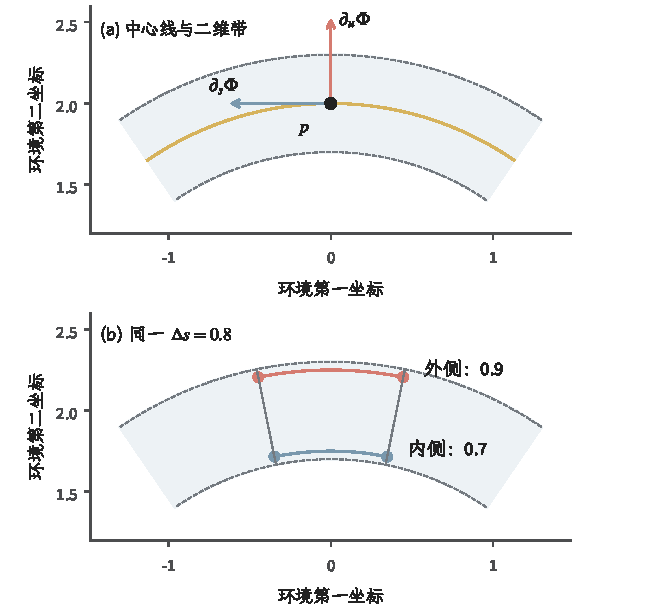
\includegraphics[width=\linewidth]{figures/math-preparation/concept-revision-linear-geometry/geometry-strip-tangent-coordinates.pdf}
 \caption{弯曲带的自由度与坐标尺度。取$R=2$、$w=0.3$。上图显示二维开带、中心线上的点$\bm p$及两个参数方向$\partial_s\Phi$、$\partial_u\Phi$，箭头仅标方向；仅把中心线作为对象时，径向方向不属于其切空间。下图取$u=-0.25$与$u=0.25$，同一坐标增量$\Delta s=0.8$对应弧长$0.7$与$0.9$。灰虚线表示不纳入开带的边界，两图等比例绘制，均为解析教学示例。}
 \label{fig:geometry-strip-tangent-coordinates}
\end{figure}

\subsection{局部PCA与切空间估计}

只有带噪观测$\bm{x}_i$时，参数化$\Phi$和潜在点$\bm{p}_i$通常都未知。此时必须先
说明要估计的潜在流形是二维带$\mathcal{M}_{\mathrm{strip}}$还是一维中心线
$\mathcal{C}$，其维数分别为$2$和$1$。局部PCA在$\bm{x}_i$附近选择观测邻居、减去
局部均值，再对局部数据矩阵做谱分解；它试图估计的是
$T_{\bm{p}_i}\mathcal{M}_{\mathrm{strip}}$或
$T_{\bm{p}_i}\mathcal{C}$。对一维中心线或一般满足$d<D$的嵌入流形，环境噪声通常
会把观测推出潜在流形，此时$T_{\bm{x}_i}\mathcal{M}$没有定义。当前二维开带则是
$\mathbb{R}^2$的开子集：足够小的扰动后$\bm{x}_i$仍在带内，并且
$T_{\bm{x}_i}\mathcal{M}_{\mathrm{strip}}=\mathbb{R}^2$；较大扰动也可能把它推出
带外。两种情形下，局部PCA要估计的潜在对象仍是$\bm{p}_i$处的切空间，而不是把观测点
直接认作生成它的潜在点。

具体地，记邻居索引集为$N_i$，选取非负权重
$\alpha_{i,j}$并令$\sum_{j\in N_i}\alpha_{i,j}=1$。局部均值和加权协方差矩阵定义为
\begin{equation}
  \overline{\bm{x}}_i
  =
  \sum_{j\in N_i}\alpha_{i,j}\bm{x}_j,
  \qquad
  \bm{C}_i
  =
  \sum_{j\in N_i}
  \alpha_{i,j}
  (\bm{x}_j-\overline{\bm{x}}_i)
  (\bm{x}_j-\overline{\bm{x}}_i)^{\top}.
  \label{eq:geometry-local-weighted-covariance}
\end{equation}
取$\bm{C}_i$最大$d$个特征值对应的特征向量张成估计切空间。这里$d$必须已知或另由
局部谱判断；权重、邻域和维数都是构造的一部分。使用局部均值可以消去邻域的一阶位置
偏移。特征向量给出的是以零速度为原点的方向子空间；若要画出局部仿射近似，可将它平移
到$\overline{\bm{x}}_i$。真实的仿射切平面应以潜在点$\bm{p}_i$为锚点，但
$\bm{p}_i$未知；因此以$\bm{x}_i$或局部均值为锚点得到的只是估计，不能称为
$\bm{x}_i$处的真实切平面。

这个结论来自局部Taylor展开。设无噪声邻居可写成
$\bm{p}_i=\varphi(\bm{z})$和
$\bm{p}_j=\varphi(\bm{z}+\bm{h})$，则
\begin{equation}
  \varphi(\bm{z}+\bm{h})-\varphi(\bm{z})
  =
  \bm{J}_{\varphi}(\bm{z})\bm{h}
  +
  O(\lVert\bm{h}\rVert_2^2).
  \label{eq:geometry-manifold-local-taylor}
\end{equation}
一阶项位于切空间，偏离切平面的法向分量由曲率通过二阶项出现。若邻域半径记为$h$，
切向位移通常为$O(h)$，曲率造成的法向位移为$O(h^2)$。因此缩小邻域可以降低曲率偏差，
却也减少可用样本，并使测量噪声相对于真实局部变化更突出。

两种潜在对象的误差机制不同。对一维中心线$\mathcal{C}$，邻域过大时切线已经随$s$
明显旋转，PCA得到的是多段切线的折中；邻域过小时，样本又可能只沿偶然方向排列。对二维
带$\mathcal{M}_{\mathrm{strip}}$，切空间在当前平面例子中就是$\mathbb{R}^2$，不能因
点带狭窄就把它改称一维流形；但当横向宽度$w$小于噪声尺度时，有限样本中的第二个内在
方向仍可能无法稳定辨认。局部谱间隙、采样密度、曲率、带宽、潜在对象和测量误差必须
共同解释，不能仅按某个固定邻居数宣布“数据维数”。

内在维数也不等于能够无失真嵌入的最小全局维数。圆是一维流形，却不能以保持其拓扑的
方式用一张实数坐标图覆盖；它可以无自交地嵌入二维平面。局部PCA回答附近有多少一阶
自由度，并不自动构造全局参数$s$，更不能保证参数化在整条点带上不重叠。

\section{约束运动的长度与方向}
\label{sec:geometry-metric-path-geodesic}

\subsection{Riemann度量}

切空间只说明哪些一阶速度可行，还没有规定不同速度有多长。同一个方向向量在不同位置也可能具有不同长度，因此内积需要按位置指定。

\begin{definition}[Riemann度量]
\label{def:geometry-riemannian-metric}
光滑流形$\mathcal M$上的\term{Riemann度量}（Riemannian metric）为每个点$\bm{p}$的切空间指定一个随
$\bm{p}$光滑变化的内积$g_{\bm{p}}$。在局部坐标
$\bm{z}=(z^1,\ldots,z^d)$中，它由对称正定矩阵
$\bm{G}(\bm{z})=[g_{i,j}(\bm{z})]$表示。对曲线$\gamma(t)=\varphi(\bm z(t))$，坐标速度
$\dot{\bm{z}}$对应的几何速度长度为
\begin{equation}
  \lVert\dot{\gamma}\rVert_g^2
  =
  \dot{\bm{z}}^{\top}
  \bm{G}(\bm{z})
  \dot{\bm{z}}.
  \label{eq:geometry-riemannian-speed}
\end{equation}
光滑变化是指这些局部矩阵的条目光滑，并在重叠坐标图中按式~\eqref{eq:geometry-metric-coordinate-transform}表示同一内积。
\end{definition}
这里的$\bm{G}$不是点坐标的协方差矩阵，也不是所有位置共享的距离学习矩阵。它描述
每个点处切向速度的局部内积，并且可以随位置变化。

嵌入流形可以继承环境空间的欧氏内积。若
$\bm{p}=\varphi(\bm{z})$，坐标速度$\dot{\bm{z}}$在环境空间中对应
$\bm{J}_{\varphi}(\bm{z})\dot{\bm{z}}$，因此诱导度量为
\begin{equation}
  \bm{G}(\bm{z})
  =
  \bm{J}_{\varphi}(\bm{z})^{\top}
  \bm{J}_{\varphi}(\bm{z}).
  \label{eq:geometry-induced-metric}
\end{equation}
Jacobian矩阵满列秩保证$\bm{G}$正定。若Jacobian矩阵退化，某个非零坐标速度会被映成零，
式~\eqref{eq:geometry-induced-metric}只能产生半正定形式，这也说明流形参数化为何要求
满秩。

由式~\eqref{eq:geometry-strip-s-tangent}和
\eqref{eq:geometry-strip-u-tangent}，弯曲点带的诱导度量为
\begin{equation}
  \bm{G}(s,u)
  =
  \begin{bmatrix}
    (1+u/R)^2 & 0\\
    0 & 1
  \end{bmatrix}.
  \label{eq:geometry-strip-metric}
\end{equation}
同样的坐标增量$\mathrm{d}s$在外侧$u>0$对应更长圆弧，在内侧$u<0$对应更短圆弧。
坐标数值相同不意味着几何长度相同，度量正是二者之间的换算规则。

\subsection{路径长度与参数化}

先设分段光滑路径$\gamma:[a,b]\to\mathcal{M}$的像完全落在一张坐标图内，并在该坐标
中写成$\bm{z}(t)$。它的长度定义为
\begin{equation}
  L_g(\gamma)
  =
  \int_a^b
  \sqrt{
    \dot{\bm{z}}(t)^{\top}
    \bm{G}(\bm{z}(t))
    \dot{\bm{z}}(t)
  }
  \,\mathrm{d}t.
  \label{eq:geometry-riemannian-curve-length}
\end{equation}
若整条路径不能落在一张坐标图内，就把$[a,b]$分成有限个子区间，使每段路径像位于一张
坐标图中，再把各段长度相加。下文的坐标变换计算说明，重叠区域采用哪张图以及怎样进一步
细分都不会改变总长度。

参数$t$只规定沿路径前进的方式。若用严格递增的光滑参数
$t=\tau(r)$重新参数化，链式法则产生因子$\tau'(r)$，它与
$\mathrm{d}t=\tau'(r)\mathrm{d}r$恰好配对，所以长度不变。停得久或走得快不会改变
已经走过的几何路线长度。

坐标变化也不会改变长度。设新坐标为$\bm{v}$，旧坐标满足
$\bm{z}=\psi(\bm{v})$，并记$\bm{A}=\bm{J}_{\psi}(\bm{v})$。速度满足
$\dot{\bm{z}}=\bm{A}\dot{\bm{v}}$。同一个内积在新坐标中的矩阵必须变为
\begin{equation}
  \widetilde{\bm{G}}(\bm{v})
  =
  \bm{A}^{\top}\bm{G}(\psi(\bm{v}))\bm{A}.
  \label{eq:geometry-metric-coordinate-transform}
\end{equation}
代入可得
\[
  \dot{\bm{v}}^{\top}\widetilde{\bm{G}}\dot{\bm{v}}
  =
  \dot{\bm{z}}^{\top}\bm{G}\dot{\bm{z}}.
\]
所以式~\eqref{eq:geometry-riemannian-curve-length}计算的是几何路径，而不是某张坐标表
上的数字长度。若只换坐标分量却不按式
~\eqref{eq:geometry-metric-coordinate-transform}变换度量，所得长度就描述了另一个
几何问题。

\subsection{沿路径比较切向方向}

度量只能直接比较同一点切空间中的向量；沿路径前进时，不同时刻的速度属于不同切空间，
仍不能直接相减。为定义“方向沿路径怎样变化”，需要一条把方向导数保留在切空间中的规则。

\begin{definition}[向量场与联络]
\label{def:geometry-connection}
\term{向量场}（vector field）
$\bm{V}$在每个$\bm{p}\in\mathcal{M}$处选取切向量
$\bm{V}(\bm{p})\in T_{\bm{p}}\mathcal{M}$。\term{联络}（connection）为两个光滑
向量场$\bm{U},\bm{V}$指定另一个向量场
$\nabla_{\bm{U}}\bm{V}$，称为$\bm{V}$沿$\bm{U}$的
\term{协变导数}（covariant derivative），并满足
\[
  \nabla_{f\bm{U}+h\bm{W}}\bm{V}
  =
  f\nabla_{\bm{U}}\bm{V}
  +
  h\nabla_{\bm{W}}\bm{V},
  \qquad
  \nabla_{\bm{U}}(a\bm{V}+b\bm{W})
  =
  a\nabla_{\bm{U}}\bm{V}
  +
  b\nabla_{\bm{U}}\bm{W},
\]
以及Leibniz规则
\[
  \nabla_{\bm{U}}(f\bm{V})
  =
  \bm{U}(f)\bm{V}
  +
  f\nabla_{\bm{U}}\bm{V},
\]
其中$f,h$为光滑函数，$a,b\in\mathbb{R}$。第一条说明求导方向可以按位置变化的
系数组合，Leibniz规则则保留普通导数的乘积法则；$\bm U(f)$表示$f$沿$\bm U$的方向导数。
\end{definition}

已有度量之后，需要选择与长度判断一致的方向导数，而不是任意增加一套比较规则。
\begin{definition}[Levi--Civita联络]
\label{def:geometry-levi-civita-connection}
给定Riemann度量$g$，同时保持度量且无挠的联络称为
\term{Levi--Civita联络}（Levi--Civita connection）。两项条件对任意光滑向量场
$\bm U,\bm V,\bm W$分别为
\[
  \bm{U}\bigl(g(\bm{V},\bm{W})\bigr)
  =
  g(\nabla_{\bm{U}}\bm{V},\bm{W})
  +
  g(\bm{V},\nabla_{\bm{U}}\bm{W}),
  \qquad
  \nabla_{\bm{U}}\bm{V}-\nabla_{\bm{V}}\bm{U}
  =
  [\bm{U},\bm{V}],
\]
其中交换子由$[\bm U,\bm V](f)=\bm U(\bm V(f))-\bm V(\bm U(f))$
对任意光滑函数$f$定义。
\end{definition}
Riemann度量唯一地确定这样的联络。“保持度量”说明沿路径比较方向时仍遵守内积的乘积法则；
“无挠”使先后交换两次方向导数产生的差异恰由上述交换子记录。
沿曲线$\gamma$的切向量场
$\bm{V}(t)$的协变导数记作
$D\bm{V}/\mathrm{d}t$。对继承环境欧氏度量的嵌入流形，它可以直观而准确地写成
\[
  \frac{D\bm{V}}{\mathrm{d}t}
  =
  \operatorname{proj}_{T_{\gamma(t)}\mathcal{M}}
  \frac{\mathrm{d}\bm{V}}{\mathrm{d}t};
\]
也就是先在环境空间求普通导数，再只保留当前切空间中的分量。这个定义使后文的“协变
加速度为零”不再依赖尚未解释的术语。

\subsection{测地距离}

\begin{definition}[测地距离]
\label{def:geometry-geodesic-distance}
在具有Riemann度量$g$的光滑流形上，若两点$\bm{p},\bm{q}\in\mathcal{M}$位于同一路径连通分支，它们之间的
\term{测地距离}（geodesic distance）定义为$\mathcal{M}$内所有分段光滑连接路径
长度的下确界：
\begin{equation}
  d_g(\bm{p},\bm{q})
  =
  \inf_{\substack{\gamma(a)=\bm{p}\\\gamma(b)=\bm{q}}}
  L_g(\gamma).
  \label{eq:geometry-geodesic-distance}
\end{equation}
若不存在连接两点的路径，则约定$d_g(\bm{p},\bm{q})=+\infty$；在整个可能不连通的
$\mathcal{M}$上，这给出的是允许取无穷值的扩展距离。
\end{definition}
它比较的是被限制在流形上的行走代价。环境空间欧氏距离允许直接穿过流形外部，所以总有
\[
  \lVert\bm{p}-\bm{q}\rVert_2
  \leq
  d_g(\bm{p},\bm{q})
\]
用于欧氏诱导度量的情形。若连接两点的欧氏直线段完全位于流形内，它就给出长度等于弦长
的候选路径，因而上式取等。反过来，只有当长度下确界确实由某条允许路径达到时，取等才会
迫使该最短路径沿直线段前进，至多相差保持方向的重参数化；下确界不取到时，即使直线段
不在流形内，两种距离仍可能相等。

现在可以明确比较中心线与二维带上的距离。取
$\bm{p}=\Phi(s,0)$和$\bm{q}=\Phi(t,0)$。若允许路径只能位于一维中心线
$\mathcal{C}$，则$s$是弧长参数，并且当前开圆弧上
\[
  d_{\mathcal{C}}(\bm{p},\bm{q})=|s-t|.
\]
若允许路径在二维带$\mathcal{M}_{\mathrm{strip}}$内移动，中心线弧只是一个候选，
路径还可以向内侧移动以缩短长度，因此只能一般地写成
\[
  \lVert\bm{p}-\bm{q}\rVert_2
  \leq
  d_{\mathcal{M}_{\mathrm{strip}}}(\bm{p},\bm{q})
  \leq
  d_{\mathcal{C}}(\bm{p},\bm{q})
  =
  |s-t|.
\]
式~\eqref{eq:geometry-strip-chord-distance}给出左端环境距离；把
$d_{\mathcal{M}_{\mathrm{strip}}}$与$d_{\mathcal{C}}$都简称为“沿带距离”会掩盖
允许路径的差别。若另把中心线闭合成完整圆，$d_{\mathcal{C}}$还要在顺时针和逆时针
两段弧长中取较小者。

为把两种距离画在同一尺度上，另取完整单位圆作为独立例子。两点夹角
$0\leq\theta\leq\pi$时，测地距离是短弧长度$\theta$，环境距离是弦长
$2\sin(\theta/2)$。$\theta=\pi/2$时分别为$\pi/2$与$\sqrt2$；小角度下
$2\sin(\theta/2)=\theta-\theta^3/24+O(\theta^5)$，因此局部两者接近，全局却有
不同的长度。完整圆允许选择两条弧，不能与前面的开圆弧或二维带的可行路径混同。

\begin{figure*}[htbp]
 \centering
 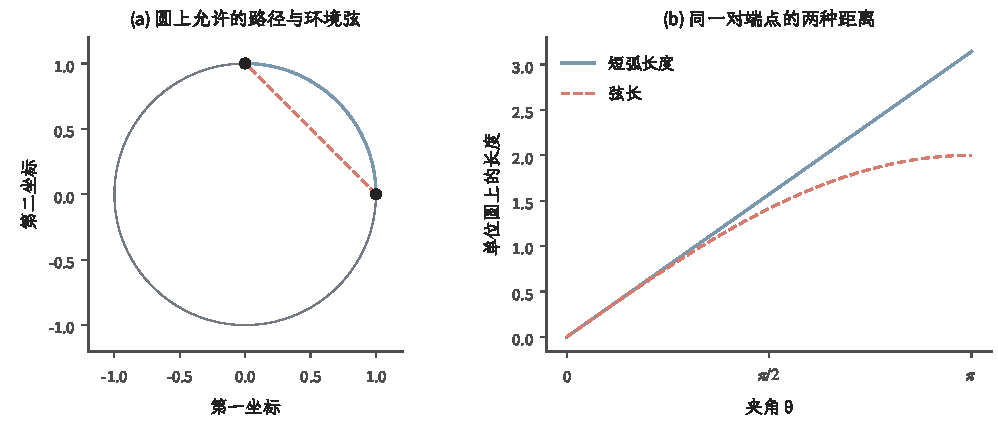
\includegraphics[width=\linewidth]{figures/math-preparation/analysis-geometry/geometry-circle-distances.pdf}
 \caption{完整单位圆上的短弧与环境弦长。左图取夹角$\pi/2$，蓝线沿圆移动，红虚线穿过圆内；右图比较全部$\theta\in[0,\pi]$的两种长度。弦在环境平面中可行，在圆上却不是允许路径。图为解析教学示例。}
 \label{fig:geometry-circle-distances}
\end{figure*}

\subsection{无切向加速度与全局最短路径}

联络建立以后，可以区分运动方向的局部条件与端点之间的全局最短要求。

\begin{definition}[测地线]
\label{def:geometry-geodesic}
对Riemann流形的Levi--Civita联络，采用仿射参数时，
\term{测地线}（geodesic）定义为协变加速度为零的曲线：
\[
  \frac{D\dot{\gamma}}{\mathrm{d}t}=\bm{0}.
\]
\end{definition}
白话地说，它的速度沿曲线作平行移动，不产生切向转弯。Levi--Civita联络在局部坐标中的
系数称为Christoffel符号：
\begin{equation}
  \Gamma^k_{i,j}
  =
  \frac12
  \sum_{\ell=1}^{d}
  g^{k,\ell}
  \left(
    \frac{\partial g_{\ell,j}}{\partial z^i}
    +
    \frac{\partial g_{i,\ell}}{\partial z^j}
    -
    \frac{\partial g_{i,j}}{\partial z^\ell}
  \right),
  \label{eq:geometry-christoffel-symbols}
\end{equation}
其中$[g^{i,j}]=\bm{G}^{-1}$。测地线条件在坐标中写成
\begin{equation}
  \ddot z^k
  +
  \sum_{i,j=1}^{d}
  \Gamma^k_{i,j}(\bm{z})\dot z^i\dot z^j
  =
  0.
  \label{eq:geometry-geodesic-equation}
\end{equation}
Christoffel符号依赖坐标，不是张量；协变导数和式
~\eqref{eq:geometry-geodesic-equation}描述的曲线才是坐标无关对象。

固定端点并对能量
\[
  E(\gamma)
  =
  \frac12\int_a^b
  \dot{\bm{z}}^{\top}\bm{G}(\bm{z})\dot{\bm{z}}
  \,\mathrm{d}t
\]
应用Euler--Lagrange方程，也会得到式~\eqref{eq:geometry-geodesic-equation}。
每条测地线在任一点附近取足够短的一段，都在该邻域内连接其端点的曲线中长度最短，但
这项局部性质不保证整段曲线在所有连接路径中最短。若一段测地线的长度等于式
~\eqref{eq:geometry-geodesic-distance}的下确界，就称它为连接两端点的
\term{长度最短测地线}（length-minimizing geodesic）。越过割点或共轭点，或者存在更短的
绕行路线时，测地线方程的解仍是测地线，却未必仍是长度最短测地线。

完整单位圆给出不需要这些高级术语的检验。以恒定角速度从$(1,0)^{\top}$走到
$(0,-1)^{\top}$，逆时针弧长为$3\pi/2$，顺时针弧长为$\pi/2$；两条圆弧都满足
一维圆上的测地线方程，只有短弧达到端点间的距离。因此满足局部运动方程并不能代替
比较所有允许路径。割点与共轭点用于进一步研究这项最短性质怎样失效，本章不依赖其判据。

下确界也不必在任意流形上达到。Hopf--Rinow定理的一项有限维结论是：若连通Riemann
流形关于测地距离完备，则任意两点之间都存在达到
式~\eqref{eq:geometry-geodesic-distance}的长度最短测地线。完备性不能省略。例如在
穿孔平面$\mathbb{R}^2\setminus\{\bm{0}\}$中，点$(-1,0)^{\top}$与$(1,0)^{\top}$
之间路径长度的下确界为$2$，路径可以任意贴近被删去的原点，却没有长度恰为$2$的允许
路径。因此这里的测地距离仍等于两点的欧氏距离$2$，但直线段不允许且下确界不取到；
这正是上述反向结论需要“下确界达到”条件的原因。局部测地线方程仍可求解，但它本身
不保证全局最短路存在。

\subsection{近邻图与测地距离近似}

对带噪观测$\bm{x}_i$，可以把每个样本连接到距离阈值$\varepsilon$内的样本，或连接到$k$个
最近邻，并以$\lVert\bm{x}_i-\bm{x}_j\rVert_2$作为边长。最短边路径试图近似的是所选
潜在流形上$\bm{p}_i$与$\bm{p}_j$之间的测地距离；潜在模型并不会自动在观测点
$\bm{x}_i$与$\bm{x}_j$之间给出测地距离，因为观测可能位于所选流形内，也可能位于其外。
潜在对象取$\mathcal{C}$还是
$\mathcal{M}_{\mathrm{strip}}$，目标距离也随之改变。这里暂时只需要“顶点、边和路径”
这些对象；一般图结构和图算法将在第~\ref{part:discrete-mathematics-and-graph-theory}
部分系统建立。

这项近似依赖两个相反要求。邻域要足够小，使每条边只跨越流形上近似平直的一段，避免从
弯曲点带的一折直接跳到另一折；邻域又要足够大，使有限样本之间能够连通。对弯曲点带，
若$\varepsilon$超过两折之间的环境间隔，最短路会产生穿带“捷径”，系统性低估测地距离。
若$\varepsilon$小于某些采样空隙，同一条连续点带又可能被拆成多个分支，距离变为无穷或
无法计算。

$k$近邻也没有消除这个取舍。稀疏区域中的第$k$个邻居可能很远，密集区域中的相同$k$
又可能只覆盖极小范围；非均匀采样还会产生方向不对称。要把最短路收敛为真实测地距离，
需要流形光滑、采样逐渐稠密、噪声受控，并让邻域尺度随样本量以合适速度缩小。具体降维
算法还要说明图构造、边权和误差条件，不能由“局部距离近似正确”直接推出全局坐标恢复
正确。

\section{平滑能量与几何算子}
\label{sec:geometry-smoothness-geometric-operators}

度量已经规定了沿路径移动多远，现在把它用于定义函数沿空间变化有多快。
微分给出每个方向的变化，度量把微分转成梯度，积分再汇总各点的变化能量；
Laplace--Beltrami算子由这同一能量的变分产生。这样，梯度、能量和算子属于同一条推导，
而不是三个孤立的几何定义。

\subsection{流形梯度}

设$f:\mathcal{M}\to\mathbb{R}$为光滑函数。它在$\bm{p}$处的微分
$\mathrm{d}f_{\bm{p}}$把切向量映为函数的一阶变化，是一个线性泛函。度量允许把这个
泛函表示成切向量。方向变化规则与表示它的梯度需要区分：前者由$f$给出，后者还用到度量。

\begin{definition}[Riemann梯度]
\label{def:geometry-riemannian-gradient}
光滑实函数$f$的\term{Riemann梯度}（Riemannian gradient）
$\operatorname{grad}f(\bm{p})\in T_{\bm{p}}\mathcal{M}$由
\begin{equation}
  g_{\bm{p}}\bigl(
    \operatorname{grad}f,\bm{v}
  \bigr)
  =
  \mathrm{d}f_{\bm{p}}(\bm{v})
  \qquad
  \text{对所有 }\bm{v}\in T_{\bm{p}}\mathcal{M}
  \label{eq:geometry-riemannian-gradient-definition}
\end{equation}
唯一确定。
\end{definition}

它依赖度量：微分描述同一个线性变化规则，采用不同内积表示时，得到的梯度
向量可以不同。

在局部坐标中，令普通偏导数组成
$\nabla_{\bm{z}}f=(\partial_1f,\ldots,\partial_df)^{\top}$。若梯度的坐标分量为
$\bm{a}$，式~\eqref{eq:geometry-riemannian-gradient-definition}要求
\[
  \bm{a}^{\top}\bm{G}\bm{v}
  =
  \nabla_{\bm{z}}f^{\top}\bm{v}
\]
对所有$\bm{v}$成立，因此
\begin{equation}
  [\operatorname{grad}f]_{\bm{z}}
  =
  \bm{G}^{-1}\nabla_{\bm{z}}f.
  \label{eq:geometry-riemannian-gradient-coordinates}
\end{equation}
不能在弯曲坐标中直接把偏导列表当作几何梯度；逆度量负责把协变量形式的微分转成切向量。

\subsection{Dirichlet能量}

在流形上积分还需要体积元素。度量矩阵把一个小坐标盒的体积缩放为
$\sqrt{\det\bm{G}(\bm{z})}$倍，因此
\[
  \mathrm{d}V_g
  =
  \sqrt{\det\bm{G}(\bm{z})}\,\mathrm{d}\bm{z}.
\]
\begin{definition}[Dirichlet能量]
\label{def:geometry-dirichlet-energy}
光滑实函数$f$的\term{Dirichlet能量}定义为
\begin{equation}
  \mathcal{E}(f)
  =
  \frac12
  \int_{\mathcal{M}}
  \lVert\operatorname{grad}f\rVert_g^2
  \,\mathrm{d}V_g.
  \label{eq:geometry-dirichlet-energy}
\end{equation}
积分若不有限，能量取$+\infty$。
\end{definition}
它累积函数在各个切向方向上的平方变化。常量函数能量为零；函数若只在很短的几何距离内
剧烈变化，能量就大。这里“平滑”是相对于度量和体积而言的，不是坐标表上逐坐标变化小
的简称。

对弯曲点带，由式~\eqref{eq:geometry-strip-metric}，
\[
  \sqrt{\det\bm{G}(s,u)}
  =
  1+\frac{u}{R},
  \qquad
  \bm{G}^{-1}(s,u)
  =
  \begin{bmatrix}
    (1+u/R)^{-2}&0\\
    0&1
  \end{bmatrix}.
\]
所以
\begin{equation}
  \mathcal{E}(f)
  =
  \frac12
  \int
  \left[
    \frac{(\partial_sf)^2}{1+u/R}
    +
    \left(1+\frac{u}{R}\right)(\partial_uf)^2
  \right]
  \,\mathrm{d}s\,\mathrm{d}u.
  \label{eq:geometry-strip-dirichlet-energy}
\end{equation}
两个方向的权重来自同一个几何：外侧单位$s$坐标更长，所以相同的$\partial_sf$对应较小
的单位几何长度变化；同时外侧的小坐标盒具有更大面积。

\subsection{Laplace--Beltrami算子}

前文的$\mathcal{M}_{\mathrm{strip}}$是无流形边界的开带。为讨论边界积分，另取它的
截断闭带
\[
  \overline{\mathcal{M}}_{\mathrm{strip}}
  =
  \{\Phi(s,u):s\in[s_-,s_+],\ |u|\leq w\}.
\]
它是紧致、具有分片光滑边界的积分域，四个角点的外法向不唯一，但这些点的边界测度为零。
以下写带边界公式时，$\mathcal{M}$表示这类积分域，$\partial\mathcal{M}$表示积分域的
边界；函数及所需导数应能从内部延拓到各段边界，从而具有相应的边界迹。

要找到能量下降的方向，令$f_{\epsilon}=f+\epsilon h$，其中$h$为光滑测试函数。对式
~\eqref{eq:geometry-dirichlet-energy}求$\epsilon=0$处导数，得到
\begin{equation}
  \left.
  \frac{\mathrm{d}}{\mathrm{d}\epsilon}
  \mathcal{E}(f+\epsilon h)
  \right|_{\epsilon=0}
  =
  \int_{\mathcal{M}}
  g(\operatorname{grad}f,\operatorname{grad}h)
  \,\mathrm{d}V_g.
  \label{eq:geometry-dirichlet-first-variation}
\end{equation}
要把导数从$h$移到$f$，需要汇总梯度场向邻域流出的变化。若光滑向量场$\bm{V}$在局部坐标中的分量为$V^1,\ldots,V^d$，其散度定义为
\[
  \operatorname{div}_g\bm{V}
  =
  \frac{1}{\sqrt{\det\bm{G}}}
  \sum_{i=1}^{d}
  \frac{\partial}{\partial z^i}
  \left(\sqrt{\det\bm{G}}\,V^i\right).
\]
把梯度代入散度，就得到由当前几何确定的二阶算子。
\begin{definition}[Laplace--Beltrami算子]
\label{def:geometry-laplace-beltrami}
在Riemann流形上，对二阶连续可微的实函数$f$，\term{Laplace--Beltrami算子}（Laplace--Beltrami operator）定义为$\Delta_gf=\operatorname{div}_g(\operatorname{grad}f)$；其坐标表达式为
\begin{equation}
  \Delta_g f
  =
  \frac{1}{\sqrt{\det\bm{G}}}
  \sum_{i,j=1}^{d}
  \frac{\partial}{\partial z^i}
  \left(
    \sqrt{\det\bm{G}}\,
    g^{i,j}
    \frac{\partial f}{\partial z^j}
  \right).
  \label{eq:geometry-laplace-beltrami}
\end{equation}
其中$[g^{i,j}]=\bm G^{-1}$。本章采用$\Delta_g$作为热方程生成元，$-\Delta_g$在适当边界条件下为非负算子。
\end{definition}
它是梯度的散度，描述函数值相对于局部几何平均的偏离。

流形上的分部积分公式现在把导数从$h$移到$f$：
\begin{equation}
  \int_{\mathcal{M}}
  g(\operatorname{grad}f,\operatorname{grad}h)
  \,\mathrm{d}V_g
  =
  -\int_{\mathcal{M}}
  h\,\Delta_g f\,\mathrm{d}V_g
  +
  \int_{\partial\mathcal{M}}
  h\,\partial_{\bm{n}}f\,\mathrm{d}S_g.
  \label{eq:geometry-green-identity}
\end{equation}
其中$\bm{n}$为边界外法向，$\partial_{\bm{n}}f$是法向导数，$\mathrm dS_g$为由度量诱导的边界面积元。

式~\eqref{eq:geometry-green-identity}也给出变分推导的边界。若积分域改为紧致无边界
流形，边界项消失；若固定$f$在边界上的迹，则允许的扰动满足$h=0$，得到Dirichlet边界
条件；若边界值自由，能量驻点自然要求$\partial_{\bm{n}}f=0$，得到Neumann边界条件。
未经说明就删去边界项，等于偷偷选择了问题。截断闭带
$\overline{\mathcal{M}}_{\mathrm{strip}}$的边界有两条长边和两个端部；采用哪种条件会
改变平滑结果。

若施加相应边界条件使边界项为零，式
~\eqref{eq:geometry-dirichlet-first-variation}表明能量关于$L^2$内积的梯度是
$-\Delta_gf$。因此热方程
\begin{equation}
  \frac{\partial f}{\partial t}
  =
  \Delta_gf
  \label{eq:geometry-heat-equation}
\end{equation}
沿时间降低Dirichlet能量并扩散局部差异。这里的$t$是扩散时间，不是点带坐标$s$；
扩散、优化迭代和物理时间在具体模型中可能对应不同对象。

能量恒等式还控制了标量谱。对正维数的紧致、光滑、无边界Riemann流形，$-\Delta_g$在
$L^2(\mathcal{M},\mathrm{d}V_g)$中具有离散非负谱
\[
  0=\lambda_0\leq\lambda_1\leq\lambda_2\leq\cdots,
  \qquad
  \lambda_k\to\infty,
\]
并可选取一组光滑特征函数构成$L^2$完备正交系。若
$-\Delta_g\phi=\lambda\phi$，由式~\eqref{eq:geometry-green-identity}取
$h=\phi$可得
\[
  \lambda\int_{\mathcal{M}}\phi^2\,\mathrm{d}V_g
  =
  \int_{\mathcal{M}}
  \lVert\operatorname{grad}\phi\rVert_g^2
  \,\mathrm{d}V_g
  \geq0,
\]
这解释了非负性；离散性与完备性还需要紧致性和椭圆算子理论。流形连通时，零能量迫使
$\operatorname{grad}\phi=\bm{0}$，故零特征空间恰由常量函数组成。带边界时必须连同
边界条件陈述谱：连通域上的Neumann条件仍保留常量零模，Dirichlet条件则使首个特征值
严格为正。

\begin{example}[圆上的坐标、能量与谱尺度]
\label{ex:geometry-circle-energy-scale}
在半径为$R$的完整圆上取角坐标$\theta$，诱导度量为$g_{\theta\theta}=R^2$，
体积元为$R\,\mathrm d\theta$。对$f(\theta)=\cos\theta$，
\[
 \begin{aligned}
 \lVert\operatorname{grad}f\rVert_g^2
   &=\frac{\sin^2\theta}{R^2},\\
 \Delta_g f&=\frac{1}{R^2}f''=-\frac{\cos\theta}{R^2},\\
 \mathcal E(f)&=\frac12\int_0^{2\pi}\frac{\sin^2\theta}{R^2}R\,\mathrm d\theta
              =\frac{\pi}{2R}.
 \end{aligned}
\]
同一幅度的函数变化放在更大的圆上，沿单位长度的变化较小，所以能量和谱特征值都下降。
若改用局部弧长坐标$s=R\theta$，度量分量变为$1$，而$f(s)=\cos(s/R)$的导数相应多出
$1/R$；结果保持不变。此处$\mathcal E$采用前文的$1/2$归一化，若省去它，能量也要同步加倍。
\end{example}

\subsection{采样密度与几何算子的离散近似}

从点云构造加权近邻图时，常用相邻函数值差
\[
  \frac12\sum_{i,j}w_{i,j}(f_i-f_j)^2
\]
近似连续Dirichlet能量。这个式子将在图拉普拉斯建立后由
第~\ref{part:discrete-mathematics-and-graph-theory}部分重新推导。此处需要先看清
连续对象：流形、度量、体积测度和函数共同决定
式~\eqref{eq:geometry-dirichlet-energy}。

样本若按非均匀密度$q(\bm{p})$取得，简单样本平均更接近对
$q\,\mathrm{d}V_g$积分，而不是对几何体积$\mathrm{d}V_g$积分。不同的核归一化可能
保留这个密度权重，也可能试图消除它，极限算子因而不同。边权非负和矩阵对称只保证某个
离散二次型非负，不足以证明它近似指定的Laplace--Beltrami算子；还要核对邻域尺度、
采样密度、边界处理和归一化。

标量函数的扩散也不能直接替代向量场扩散。前文定义的Levi--Civita联络先把不同点处
切向量的变化转成协变导数；在此基础上，可以用
$\int_{\mathcal{M}}\lVert\nabla\bm{V}\rVert_g^2\,\mathrm{d}V_g$
衡量向量场变化，并由其变分定义联络拉普拉斯
$\nabla^{*}\nabla$。这里$\nabla^{*}$表示相对于$L^2$内积的伴随；不同文献对拉普拉斯
整体符号可能采用相反约定。该构造先规定跨点比较，再累积变化，不能把标量
Laplace--Beltrami公式逐坐标照搬。第
~\ref{part:discrete-mathematics-and-graph-theory}部分建立离散Dirichlet能量和图谱时，
还要分别核对边权、归一化与采样密度对应哪个连续算子。

\section{变换群、不变性与等变性}
\label{sec:geometry-group-invariance-equivariance}

平滑性比较邻近点，对称性则比较一组指定变换前后的对象。
例如旋转坐标可能只改表示，旋转一幅观测图像却会改输入；要求输出保持不变还是随之变换，
取决于任务。下面先规定变换复合与其作用，再讨论函数可以满足的响应条件。

\subsection{群作用}

坐标可以改变，点带也可以在平面中整体旋转；我们需要区分“变换有哪些代数关系”和
“变换具体作用于什么对象”。能复合、能撤销的变换需要一套共同的代数规则。

\begin{definition}[群]
\label{def:geometry-group}
\term{群}（group）$G$是带有复合运算的集合，满足复合
封闭、结合律，具有恒等元$e$，并且每个$g\in G$都有逆元$g^{-1}$。群元素本身可以是
旋转、平移、置换或更抽象的变换。
\end{definition}

群规定复合的规则，具体的对象对应关系还要另行给出\scite{math-lee2013smooth}

\begin{definition}[群作用]
\label{def:geometry-group-action}
\term{群作用}（group action）把每个$g\in G$对应到对象空间$\mathcal{X}$上的变换，
记为$g\cdot x$，并要求
\begin{equation}
  e\cdot x=x,
  \qquad
  (g_1g_2)\cdot x
  =
  g_1\cdot(g_2\cdot x).
  \label{eq:geometry-group-action}
\end{equation}
这两个等式对所有$x\in\mathcal X$和$g_1,g_2\in G$成立。
\end{definition}
第二条保证群中的复合与实际连续施加变换一致。只列出若干数据增强而不说明复合后是否仍
在允许集合中，通常还没有定义一个群。

当作用对象是向量，且每次变换都保持线性组合时，可以把作用写成可逆线性算子。

\begin{definition}[线性表示]
\label{def:geometry-linear-representation}
\term{线性表示}（linear representation）是群在向量空间$V$上的线性作用，即映射
$\rho:G\to\operatorname{GL}(V)$满足
\begin{equation}
  \rho(e)=\bm{I},
  \qquad
  \rho(g_1g_2)=\rho(g_1)\rho(g_2).
  \label{eq:geometry-linear-representation}
\end{equation}
其中$\operatorname{GL}(V)$为$V$上全部可逆线性算子组成的群。
\end{definition}
输入与输出可以使用不同表示。例如输入点坐标按旋转矩阵变化，标量输出使用
$\rho(g)=1$，向量输出则可使用同一个旋转矩阵。后文写
$F(g\cdot x)=\rho(g)F(x)$时，$\rho$明确规定的是输出怎样响应，并不要求输出空间与
输入空间相同。

二维旋转构成群$\mathrm{SO}(2)$。角度$\theta$对应
\begin{equation}
  \bm{R}(\theta)
  =
  \begin{bmatrix}
    \cos\theta&-\sin\theta\\
    \sin\theta&\cos\theta
  \end{bmatrix},
  \qquad
  \bm{R}(\theta_1)\bm{R}(\theta_2)
  =
  \bm{R}(\theta_1+\theta_2).
  \label{eq:geometry-planar-rotation-group}
\end{equation}
它可作用于单个点、整组点、图像坐标或向量场，但这些是不同的对象空间。对弯曲点带整体
旋转时，点坐标变为$\bm{R}(\theta)\Phi(s,u)$，内在坐标$(s,u)$可以保持不变。环境
坐标改变不等于流形上的点身份或局部坐标必须改变。

有限集合$\{1,\ldots,n\}$的全部置换构成对称群$S_n$。若
$\pi\in S_n$，其置换矩阵$\bm{P}_{\pi}$可以重排点云矩阵的行。这里改变的是记录顺序，
不是把空间中的点移动到另一个几何位置。旋转和重编号都能写成矩阵乘法，却作用在不同
索引上，不能因公式外形相似就视为同一种对称。

\subsection{不变性与等变性}

\begin{definition}[不变映射]
\label{def:geometry-invariant-map}
设群$G$作用于输入空间$\mathcal{X}$。函数
$f:\mathcal{X}\to\mathcal{Y}$若满足
\begin{equation}
  f(g\cdot x)=f(x)
  \qquad
  \text{对所有 }g\in G,\ x\in\mathcal{X},
  \label{eq:geometry-invariant-map}
\end{equation}
就称为对该作用\term{不变}（invariant）。
\end{definition}

它把同一轨道
$\{g\cdot x:g\in G\}$上的输入映到相同输出。点带的总长度在整体旋转下不变，点集
分类若与记录顺序无关，也应对行置换不变。

如果输出本身带方向或位置，忽略全部变换信息会破坏对象对应关系，因而需要让输出同步变换。

\begin{definition}[等变映射]
\label{def:geometry-equivariant-map}
若输出空间$\mathcal{Y}$也有一个群作用$\rho(g)$，映射
$F:\mathcal{X}\to\mathcal{Y}$满足
\begin{equation}
  F(g\cdot x)
  =
  \rho(g)F(x),
  \label{eq:geometry-equivariant-map}
\end{equation}
对所有$g\in G$和$x\in\mathcal X$成立，就称为\term{等变}（equivariant）。
\end{definition}

白话地说，输入怎样变，输出按预先规定的对应方式
一起变。对点坐标施加旋转时，返回局部切向量的映射应让切向量也乘
$\bm{R}(\theta)$；若强迫它保持数值不变，方向就不再对应旋转后的几何对象。

不变性不是比等变性“更强”的统一目标。标量类别、位置坐标、分割掩码和向量场需要的
输出行为不同。等变映射后接一个对输出作用不变的汇总，可以得到不变输出；反过来，不变
表示已经丢弃轨道内位置，通常无法恢复一个随变换移动的输出。

对点云$\bm{X}\in\mathbb{R}^{n\times d}$，逐点共享映射
$F(\bm{X})_{i,:}=\phi(\bm{X}_{i,:})$满足
\[
  F(\bm{P}_{\pi}\bm{X})
  =
  \bm{P}_{\pi}F(\bm{X}),
\]
所以对行置换等变。再按行求和
$f(\bm{X})=\sum_i\phi(\bm{X}_{i,:})$，便有
$f(\bm{P}_{\pi}\bm{X})=f(\bm{X})$，得到置换不变性。这个例子只证明结构关系；求和
表示是否足以区分任务需要的点集，还要另行分析。

平移卷积给出另一个可直接核对的等变例子。在整个$\mathbb{R}^d$上定义
$(T_{\bm{a}}f)(\bm{x})=f(\bm{x}-\bm{a})$，并设
$k,f\in L^1(\mathbb{R}^d)$。卷积积分对几乎处处的$\bm{x}$有定义，变量替换给出
\begin{align}
  \bigl(k*(T_{\bm{a}}f)\bigr)(\bm{x})
  &=
  \int_{\mathbb{R}^d}
  k(\bm{x}-\bm{y})f(\bm{y}-\bm{a})\,\mathrm{d}\bm{y}\\
  &=
  (k*f)(\bm{x}-\bm{a})
  =
  \bigl(T_{\bm{a}}(k*f)\bigr)(\bm{x}).
  \label{eq:geometry-translation-convolution-equivariance}
\end{align}
因此理想连续域上的卷积与平移作用对几乎处处的$\bm{x}$可交换。若进一步假设相关卷积
积分在每个点都绝对收敛，例如一个函数连续且有界、另一个函数可积，则等式可以逐点理解。
有限图像若采用零填充，平移后有些值会跨出边界，等式一般不再对全部平移成立；周期边界、
有效区域或离散循环平移对应的是不同作用，必须按实际定义重新核对。

\begin{table*}[htbp]
 \centering\small
 \begin{tabularx}{\linewidth}{@{}lXX@{}}
 \toprule
 输入作用 & 不变输出 & 等变输出及其作用\\
 \midrule
 平面旋转$\bm x\mapsto\bm R\bm x$ & $\lVert\bm x\rVert_2$，数值不变 & $F(\bm x)=\bm x$，输出也乘$\bm R$\\
 点记录行置换$\bm X\mapsto\bm P\bm X$ & 行求和，汇总值不变 & 逐行共享映射，输出行也乘$\bm P$\\
 全空间信号平移 & 在可积条件下的全空间积分 & 与固定可积核卷积，输出信号同样平移\\
 \bottomrule
 \end{tabularx}
 \caption{不变性与等变性由输入、输出作用共同规定。表中的全空间信号结论不自动适用于有裁剪、边界填充或下采样的有限窗口。}
 \label{tab:geometry-invariance-equivariance}
\end{table*}

\subsection{群平均与不变函数}

对有限群，可以从任意标量函数$h:\mathcal{X}\to\mathbb{R}$构造
\begin{equation}
  \overline{h}(x)
  =
  \frac{1}{|G|}
  \sum_{g\in G}h(g\cdot x).
  \label{eq:geometry-finite-group-averaging}
\end{equation}
对任意$a\in G$，
\[
  \overline{h}(a\cdot x)
  =
  \frac{1}{|G|}
  \sum_{g\in G}h((ga)\cdot x).
\]
当$g$遍历$G$时，$ga$也恰好遍历$G$，所以右端等于$\overline{h}(x)$。这完整证明了
群平均的不变性。连续紧群可用保持群平移的Haar概率测度把求和改成积分，但非紧群没有
有限均匀概率测度，不能无条件照搬“对全部平移取平均”。

群平均也会丢失信息。若任务输出必须指出点带朝向，把所有旋转响应平均成一个标量会消除
所需方向。数据增强只在有限样本上鼓励近似关系；架构等变性则在精确算术和所声明作用下
给出结构恒等式。离散网格插值、边界填充和数值误差仍可能破坏连续旋转或平移关系，实际
实现需要按离散对象重新核对。

\subsection{旋转复合与相对位置}

一维平移群可作用于序列位置：位置同时增加$a$时，相对位移$t-s$不变。旋转位置编码把
标量位置映成若干二维旋转块。对一个频率$\omega$，令
\[
  \bm{R}_{\omega}(t)
  =
  \begin{bmatrix}
    \cos(\omega t)&-\sin(\omega t)\\
    \sin(\omega t)&\cos(\omega t)
  \end{bmatrix}.
\]
正交性与旋转复合给出
\begin{equation}
  \bm{R}_{\omega}(s)^{\top}\bm{R}_{\omega}(t)
  =
  \bm{R}_{\omega}(t-s).
  \label{eq:geometry-rotary-relative-position}
\end{equation}
因此，对二维向量$\bm{q},\bm{k}$，
\begin{equation}
  \bigl(\bm{R}_{\omega}(s)\bm{q}\bigr)^{\top}
  \bigl(\bm{R}_{\omega}(t)\bm{k}\bigr)
  =
  \bm{q}^{\top}\bm{R}_{\omega}(t-s)\bm{k}.
  \label{eq:geometry-rotary-dot-product}
\end{equation}
旋转后的内积只通过相对位移依赖$s,t$。多个频率块并置后仍保持这一性质。

这个推导说明的是位置表示的代数关系，不表示任意注意力网络都自动只使用相对位置。
查询、键之外的偏置、边界处理、截断窗口和其他位置特征都可能引入绝对位置依赖。频率
还会带来周期性：相差某些周期的位置在单个旋转块中无法区分，需要多频率组合及具体长度
范围共同判断。式~\eqref{eq:geometry-rotary-relative-position}是等变结构的依据，
不是无限长度下无碰撞编码的保证。

\section{局部关系与拓扑信息}
\label{sec:geometry-local-relations-topology}

\subsection{连通性与环}

两条互不相交的圆弧在每个内部点附近都像一条直线，一条闭合圆在每个点附近也像一条
直线。它们的局部维数和切空间类型相同，整体关系却不同：前者有两个连通分支，后者只有
一个分支并包含一条不可在圆内连续收缩到点的环。研究连续变形下保持的整体性质，需要
\term{拓扑}（topology）提供不同于长度和角度的语言。

微分几何与拓扑回答的问题不能互相替代。度量可以区分路径长短和曲率尺度，拓扑只关心
连续连接、孔洞等在连续变形下是否保留。把弯曲点带整体拉直可能大幅改变环境距离，却不
改变其连通性；把开点带的两端粘合成环则改变拓扑，即使粘合处可以做得局部平滑。

有限点本身是离散集合，若不增加邻接规则，每个点都是独立连通分支。要从点云推测连续
形状，必须选择一个尺度，把哪些局部关系视为可靠连接。这个尺度是建模条件，不是数据中
无条件存在的唯一答案。

\subsection{单纯复形}

$k$维\term{单纯形}（simplex）的几何形式，是$k+1$个仿射独立顶点的凸包；其组合形式
只记录这些顶点组成的集合。顶点是零维单纯形，边是一维单纯形，填充三角形是二维单纯形。
仿射独立保证几何单纯形确实具有维数$k$，而组合表示用于保留哪些面已被纳入。只知道三条边还不足以判断三角区域是否填满；为记录更高阶的填充，需要规定面与子面一起存在。

\begin{definition}[抽象单纯复形]
\label{def:geometry-simplicial-complex}
一个
\term{抽象单纯复形}（abstract simplicial complex）
$\mathcal{K}$是有限顶点集合上的一族非空子集，并满足向下封闭：
\begin{equation}
  \sigma\in\mathcal{K},\quad
  \varnothing\neq\tau\subseteq\sigma
  \quad\Longrightarrow\quad
  \tau\in\mathcal{K}.
  \label{eq:geometry-simplicial-complex-closure}
\end{equation}
顶点数为$k+1$的元素称为$k$维单纯形。
\end{definition}
因此，加入一个填充三角形时，它的三条边和三个顶点必须同时存在。三条边形成的空心三角
环与一个填充三角形拥有相同的一维边图，却具有不同的二维信息；高阶单纯形明确记录局部
区域已经被填充，而不是只记录成对接近。

给定点云与边距离尺度$\varepsilon>0$，可以按球的交集或成对距离构造两种不同复形。

\begin{definition}[Čech复形与Vietoris--Rips复形]
\label{def:geometry-cech-rips-complexes}
一种构造是以每个点为中心放置半径
$\varepsilon/2$的欧氏开球。只要一组球有共同交集，就把对应顶点加入同一个单纯形，得到
\term{Čech复形}（Čech complex）。两点连边表示两个球相交；按这里的开球
约定，这等价于两点距离小于$\varepsilon$。
Vietoris--Rips复形则纳入所有满足任意两顶点距离不超过$\varepsilon$的非空顶点子集。
\end{definition}

三个点形成Čech填充三角形要求三个球具有共同交集。对欧氏空间中的球，这些交集为凸集；在覆盖满足相应良好条件时，神经引理说明复形与球并集具有相同的同伦类型。这个结论解释了组合对象为何可能反映连续覆盖，但它依赖覆盖集合及其交集的条件。

Vietoris--Rips复形可以由边图直接补全高阶单纯形，计算更方便，却不等同于要求全部
球有共同交集。两种复形在尺度常数下可以互相夹住，但不能在同一阈值上不加说明地互换。

例如取$\varepsilon=1$、边长为$0.9$的正三角形。任意两顶点距离小于$1$，
所以三对半径$0.5$的开球都相交，Rips复形包含填充三角形；但覆盖三个顶点所需的
最小球半径为$0.9/\sqrt3>0.5$，三球没有共同交点，Čech复形只有三条边。
这不是开球与闭球边界约定造成的差异，而是两两接近不足以保证整体共同交集。
图~\ref{fig:geometry-cech-rips-intersection}固定这组三点和同一阈值，展示两种构造所检查的条件。
\begin{figure}[htbp]
 \centering
 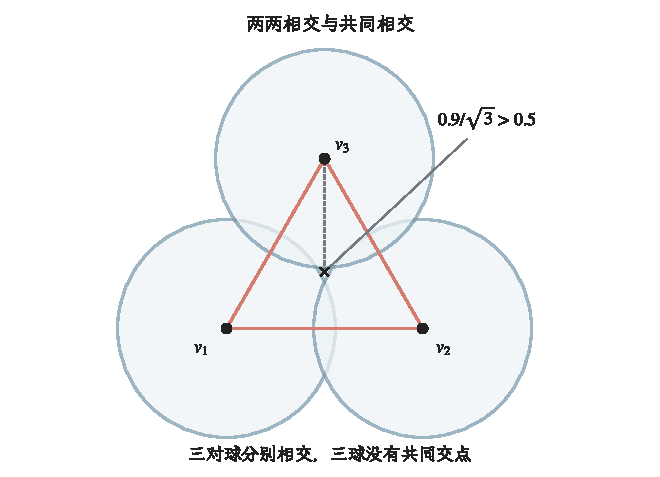
\includegraphics[width=\linewidth]{figures/math-preparation/reader-revision-linear-probability/geometry-cech-rips-intersection.pdf}
 \caption{两两距离不能替代共同交集。正三角形边长为$0.9$，阈值$\varepsilon=1$，每个蓝色开球的半径为$0.5$。红色三条边均符合两种复形的连边条件；Čech构造不纳入二维面，Rips构造纳入二维面。中心叉号到三顶点的距离均为$0.9/\sqrt3>0.5$，它给出最小覆盖半径，说明三球没有共同交点。圆周仅标出不属于开球的边界；图为解析教学构造。}
 \label{fig:geometry-cech-rips-intersection}
\end{figure}

\subsection{边界算子与同调}

要把“首尾相接”和“被一个面填充”分开，需要记录单纯形的方向。选定顶点次序后，以
$[v_0,\ldots,v_k]$表示有向$k$维单纯形；交换两个顶点会使符号反转。有限个有向
$k$维单纯形的实系数线性组合称为$k$维链，全部这些链构成向量空间$C_k(\mathcal K;\mathbb R)$。边界算子$\partial_k:C_k\to C_{k-1}$在$k\geq1$时按交替符号删除一个顶点：
\begin{equation}
  \partial_k[v_0,\ldots,v_k]
  =
  \sum_{i=0}^{k}
  (-1)^i
  [v_0,\ldots,\widehat{v_i},\ldots,v_k],
  \label{eq:geometry-simplicial-boundary}
\end{equation}
其中尖帽表示删去该顶点，算子再按线性延伸到全部链。这里采用非约化同调，约定$C_{-1}=\{0\}$和$\partial_0=0$；因此每个零维链都是闭链。

连续取两次边界总得到零，即对$k\geq1$有
\begin{equation}
  \partial_{k-1}\partial_k=0.
  \label{eq:geometry-boundary-squared-zero}
\end{equation}
证明只需跟踪任意两个被删去的顶点$v_i,v_j$。若先删$v_i$再删$v_j$，与先删$v_j$
再删$v_i$会得到同一个$(k-2)$维面；由于第二次删除时的索引相差一位，两项符号相反，
因而成对抵消。这个恒等式保证每个高维面的边界本身都没有边界。

边界一定没有边界，但并非每条闭合的链都已被某个面填充。要数出真正留下的环，就把相差一个高维边界的闭链视为同一对象。

\begin{definition}[闭链、边界与同调空间]
\label{def:geometry-homology-space}
设$\mathcal K$为有限单纯复形，$k\geq0$为整数。满足$\partial_kc=0$的$k$维链称为\term{闭链}（cycle）；存在$(k+1)$维链$b$使$c=\partial_{k+1}b$的链称为\term{边界}（boundary）。由$\partial_k\partial_{k+1}=0$，边界空间包含在闭链空间中。第$k$个实系数\term{同调空间}（homology space）为商空间
\[
 H_k(\mathcal K;\mathbb R)
 =\ker\partial_k/\operatorname{im}\partial_{k+1},\qquad
 \beta_k=\dim H_k(\mathcal K;\mathbb R).
\]
两个闭链代表同一同调类，当且仅当它们的差是一个边界；$\beta_k$称为第$k$个\term{Betti数}（Betti number）。这里的商空间采用定义~\ref{def:linear-algebra-quotient-space}，被忽略的子空间为$\operatorname{im}\partial_{k+1}$。
\end{definition}

一维中，闭链的“没有边界”表示没有未抵消的端点，边界则表示闭链已经被二维面填充。对三个顶点，令
\[
  \mathcal{K}_{\mathrm{loop}}
  =
  \{\{1\},\{2\},\{3\},
    \{1,2\},\{2,3\},\{1,3\}\},
\]
并取一维链
\[
  c=[1,2]+[2,3]-[1,3]
\]
满足$\partial_1c=0$。在$\mathcal{K}_{\mathrm{loop}}$中没有二维单纯形可产生$c$，
所以它是未填充的环；加入$[1,2,3]$后，
$c=\partial_2[1,2,3]$，同一圈边变成一个面的边界。第
~\ref{part:discrete-mathematics-and-graph-theory}部分只用顶点和边建立一般图时，不能
仅凭三条边判断三角区域是否已经填充。

图~\ref{fig:geometry-cycle-filled-simplex}固定顶点与边，只增加一个二维面。空心三角形的$\beta_0=1$、$\beta_1=1$；加入填充面后$\beta_0$仍为$1$，而$\beta_1=0$。一维边图看不到这一改变，单纯复形和边界算子却能记录它。

\begin{figure}[htbp]
 \centering
 % Two finite simplicial complexes with the same vertices and edges.
% Intended canvas: 112 mm by 36 mm. Exact combinatorial teaching construction.
\begin{tikzpicture}[x=1cm,y=1cm,font=\figurefont\small,text=FigureInk,
  line width=1.1pt,draw=FigureStroke]
 \path[use as bounding box] (0,0) rectangle (11.2,3.6);
 \begin{scope}[shift={(1.3,0.75)}]
  \coordinate (a) at (0,0); \coordinate (b) at (2.4,0);
  \coordinate (c) at (1.2,1.75);
  \draw (a)--(b)--(c)--cycle;
  \foreach \v in {a,b,c} \fill[FigureInk] (\v) circle (1.3pt);
  \node[below] at (a) {$1$}; \node[below] at (b) {$2$};
  \node[above] at (c) {$3$};
  \node at (1.2,2.5) {空心三角环};
  \node at (1.2,-0.55) {$\beta_1=1$};
 \end{scope}
 \begin{scope}[shift={(7.0,0.75)}]
  \coordinate (a) at (0,0); \coordinate (b) at (2.4,0);
  \coordinate (c) at (1.2,1.75);
  \fill[FigureYellowFill] (a)--(b)--(c)--cycle;
  \draw (a)--(b)--(c)--cycle;
  \foreach \v in {a,b,c} \fill[FigureInk] (\v) circle (1.3pt);
  \node[below] at (a) {$1$}; \node[below] at (b) {$2$};
  \node[above] at (c) {$3$};
  \node at (1.2,2.5) {填充三角面};
  \node at (1.2,-0.55) {$\beta_1=0$};
 \end{scope}
\end{tikzpicture}%

 \caption{同一圈边在两个复形中的不同含义。左侧没有二维面，闭链$c=[1,2]+[2,3]-[1,3]$不是边界；右侧纳入$[1,2,3]$，于是$c=\partial_2[1,2,3]$。填充只改变高阶面集合，顶点与边保持相同。图为组合教学示例，不表示观测点云的真实拓扑。}
 \label{fig:geometry-cycle-filled-simplex}
\end{figure}

\subsection{邻域尺度与拓扑变化}

当前二维开带$\mathcal{M}_{\mathrm{strip}}$与开矩形同胚，合适的小尺度应沿带形成一个
连通的狭长复形，并在局部三角面填充后不留下贯穿全局的环。若把一维中心线
$\mathcal{C}$的两端闭合，得到的对象是圆；若同时保留横向坐标$u$，二维带则变成环带。
两种闭合对象的维数不同，但都在合适尺度下保留一条绕中心的环。这条环不是某个单独邻域
能够识别的，它由许多局部边沿全局首尾相接形成。

尺度过小时，采样间隙使复形碎成许多连通分支；尺度增大后，相邻样本连接，真实分支逐渐
形成；尺度继续增大，跨越点带弯折的边会制造捷径，高阶单纯形还会填平原有环。因而单个
尺度上的孔洞既可能来自真实整体结构，也可能来自采样空隙。持续同调等方法会跟踪结构在
一系列尺度上的出现与消失，本章只建立其输入对象和判断边界。

前一小节的两个三点复形也说明，顶点数和边数相同仍不足以判断环是否已被填充。Euler示性数
\[
  \chi
  =
  N_0-N_1+N_2-\cdots
\]
在前者为$3-3=0$，后者为$3-3+1=1$，提供了一个粗略整体摘要。不过相同Euler示性数
也可能对应不同拓扑，不能用一个标量替代连通分支、环和更高维孔洞的分别分析。

\subsection{模糊关系与概率语义}

硬阈值会让距离略跨过$\varepsilon$的一对点从完全连接突然变成完全不连接。另一种做法为边赋予
隶属强度$\mu_{i,j}\in[0,1]$，表示在所选局部尺度下，这对点作为邻接关系的支持程度。
高阶单纯形的强度可以由边强度按某种规则组合，例如取最小值；具体组合规则属于构造定义，
需要在使用前说明。

两份关系强度还可以用
\begin{equation}
  a\mathbin{\sqcup}b
  =
  a+b-ab,
  \qquad
  a,b\in[0,1],
  \label{eq:geometry-fuzzy-union}
\end{equation}
作为一种“合并”规则。因为
$a+b-ab=1-(1-a)(1-b)$，结果仍在$[0,1]$内；该运算交换、
结合，以$0$为恒等元，并在任一输入为$1$时输出$1$。这些代数性质说明它适合作为一种
明确定义的软并集，却不表示$a$和$b$已经是两个独立事件的概率。只有先给出随机试验和
联合分布，概率加法公式中的乘积项才具有相应解释。

数值落在$[0,1]$不使$\mu_{i,j}$自动成为概率。概率要求先定义随机试验、事件和概率
测度，并满足相应的边缘与联合一致性；模糊隶属度则可以只是“多大程度上属于某种关系”
的确定性评分。把局部核权重、相似度、置信度和事件概率都称为概率，会把不同的校准要求
和组合规则混在一起。第~\ref{part:probability-stochastic-processes-statistics}部分建立
概率对象后，才能进一步比较这些解释。

UMAP等流形学习方法会从局部距离构造带强度的邻接关系，再寻找低维表示以匹配相应关系。
本节提供理解这类构造所需的坐标、度量、邻接和模糊组合语言；具体目标、优化过程及误差
证据留给\BookChapterRef{chap:dimensionality-reduction}{第三卷“模型”的“降维”章}。
低维图像中出现一个分离簇或孔洞，
不足以证明原数据具有对应任务语义，也可能受到邻居数、距离缩放、初始化和优化误差影响。

若需要把局部构造本身作为可复合对象继续抽象，可以使用\term{范畴}（category）的语言：
范畴包含对象、对象之间的箭头、每个对象的恒等箭头以及满足结合律的箭头复合；函子则在
保持恒等与复合的前提下把一个范畴映到另一个范畴。这里可以把坐标图、局部关系或它们之间
保持结构的映射组织起来，但本章关于距离、能量和单纯边界的推导都不依赖范畴论。这个入口
只说明可进一步组合的对象需要遵守什么形式规则，不把抽象名称当作额外结论。

拓扑方法同样不能修复错误的局部关系。若环境距离在弯曲点带两折之间加入大量捷径，复形
会忠实组合这些错误边；若采样完全漏掉一段区域，组合对象也无法辨认那里原本应当连接。
局部几何估计、采样覆盖和组合尺度共同限定可以支持的整体结论。

\section{本章小结}
\label{sec:geometry-summary}

弯曲点带说明，几何表示需要持续区分二维带、一维中心线、无噪声潜在点与带噪观测。点间
欧氏距离经双重中心化可恢复所给点集的中心化Gram矩阵；半正定谱给出欧氏嵌入及其最小
维数，但坐标仍可整体平移、旋转或反射。这个过程不会自动从观测距离恢复潜在点。在已有
坐标中做PCA与从距离重构坐标因此不是同一个问题；中心线测地距离与二维带测地距离也因
允许路径不同而不能混用。

流形用局部坐标描述附近自由度，切空间收集潜在点处可实现的一阶速度。坐标分量随坐标图
改变，切向量及其几何含义不应改变；局部PCA只能在潜在对象、曲率、邻域、密度和噪声
条件合适时，从观测估计潜在切方向。Riemann度量进一步在每个切空间规定长度，路径积分
把局部长度连接成整体距离；联络和协变导数则规定怎样比较不同点处的方向，并据此定义
测地线。离散近邻最短路只有在既无跨折捷径又保持采样连通时，才可能近似所选潜在流形的
测地距离。

同一度量还决定函数平滑性的含义。Riemann梯度、几何体积和Dirichlet能量通过变分关系
产生Laplace--Beltrami算子，边界条件与采样密度会改变实际平滑问题。离散图能量是这些
连续对象的一种近似入口，不是仅凭边权形式就自动成立的对应。

对称性处理的是变换下的关系。群规定变换怎样复合，群作用说明它们怎样改变具体对象；
不变映射忽略轨道内变化，等变映射让输出按规定作用同步变化。旋转、平移和节点重编号
作用于不同对象，不能只因都可写成矩阵就混为一谈。旋转位置编码的相对位移关系来自旋转
复合，但其周期、边界和其他网络部件仍限定最终行为。

局部坐标和切空间看不到整体连通与环，单纯复形通过点、边和高阶面组合局部关系。所得
拓扑依赖采样与尺度，模糊隶属强度也不自动具有概率含义。由此，本章对开篇问题的回答是：
弯曲空间不能靠一组全局线性坐标完整描述，需要把局部坐标、切空间、度量、路径、变换和
整体连接分别建模，再说明它们如何协作。第~\ref{part:discrete-mathematics-and-graph-theory}
部分将把连续平滑与离散图谱连接起来；概率分布上的局部度量则留到信息论与统计几何章节，
并继续区分几何接近与任务语义。在此之前，第~\ref{chap:probability-theory}章将先建立
随机变量、条件分布与有限样本误差的共同语言，使“观测到的点带”能够进入统计推断。
